\section{Overview}
This chapter presents a general overview of the system architecture.
The description will concentrate on the logical and physical components that
we choose in order to build our system. \\
We will start by illustrating the \textit{High Level components} of the system and their interactions. \\
Then, the section \textit{Components view} will focus on describing the single components and their interfaces. \\
The \textit{Deployment view} will provide the strategy we adopted to deploy the system, highlighting the load division between different tiers of the system. \\
In the \textit{Runtime view} we will illustrate different examples of interaction between the components with the use of Sequence Diagrams. \\
The \textit{Component interfaces} section contains a description of the interfaces provided by the logical components. \\
The chapter ends with a selection of \textit{Architectural styles and patterns} and \textit{Other design decisions} chosen while composing the application.
\clearpage

\section{High Level Components and their interactions}
The following image illustrates the general architecture on which the system will be based on. Every component can be associated with one of three logical tier: Data, Application, Presentation. \\
This is a standard and well accepted architecture, that will promote the independence between logically separated components. \\
During the design phase of the application, our focuses are the ones illustrated in the RASD document: maintainability, security, reliability and availability. \\
Given the nature of the two applications, a robust design of the Data tier is fundamental for the success of the project. \\
All the information related to the system will be stored in multiple databases. These will be protected from external attacks by a firewall and will be regularly subjected to back-up procedures. \\
The Application tier contains the logic that controls the core services of Data4Help and AutomatedSOS. The applications will be installed on different servers, located in a demilitarized zone. \\
To conclude the general description, the Presentation tier contains the system interface to the external world. The applications will be accessible both by mobile applications and web browsers. \\
Users accessing the applications via internet browsers will interact with a web server that will provide the web interface. The mobile applications instead will communicate directly with the application server. \\

\begin{figure}[ht]
    \centering
    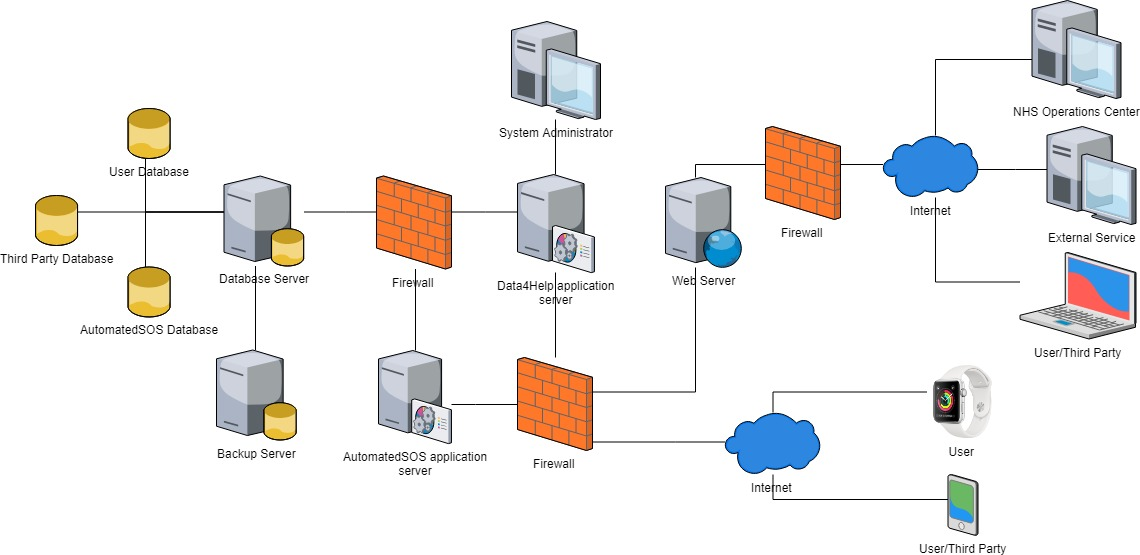
\includegraphics[width=300pt]{images/Overview.jpg}
    \caption{Overview.}
\end{figure}

\clearpage
\noindent The UML diagram below describes the main logical components that compose the system and the connections between them.
Every component enclose a specific group of services offered by the system and is not intended as a node of the physical architecture. \\
Even if this is a very high-level representation of the system it's possible to identify a general subdivision in client-related services, back-end logic and data management components. \\
A more detailed description of each component will be given in the next section. \\

\begin{figure}[ht]
    \centering
    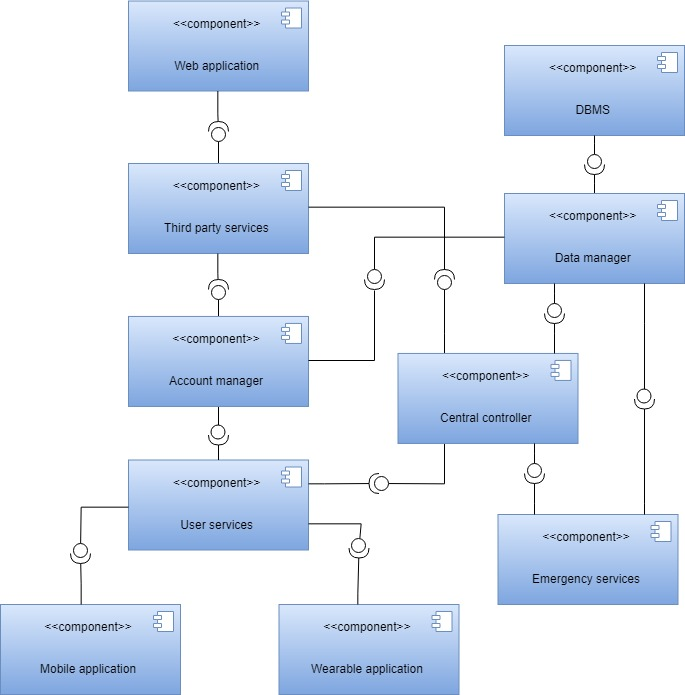
\includegraphics[width=300pt]{images/High-Level_Components.jpg}
    \caption{High Level Components.}
    \label{HLC}
\end{figure}
\clearpage

\hypertarget{CV}{\section{Component	View}}
\begin{figure}[ht]
    \centering
    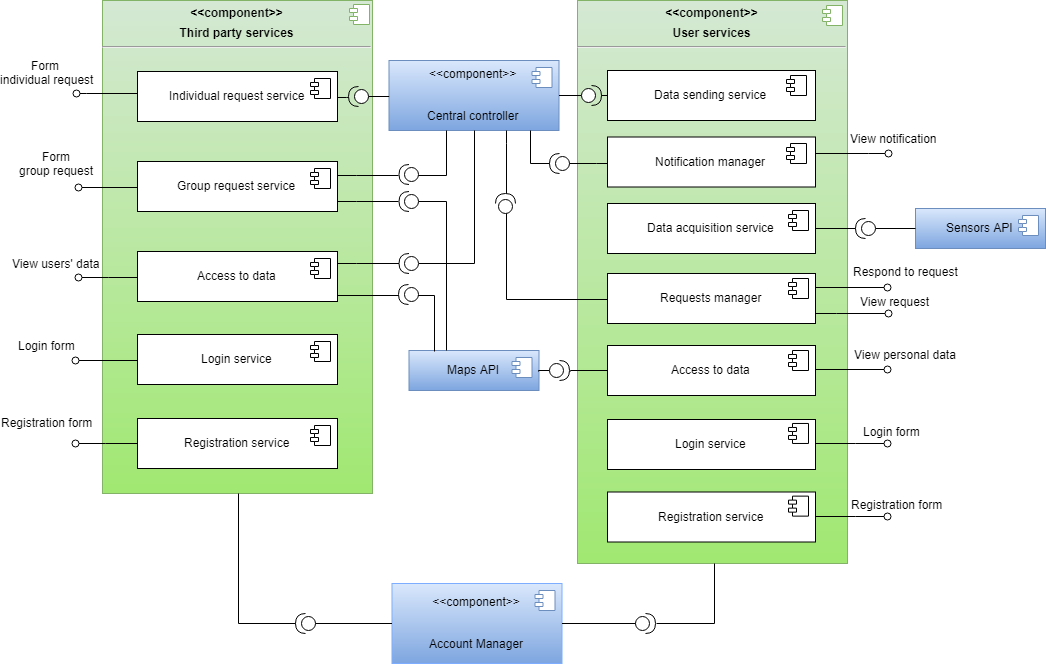
\includegraphics[width=345pt]{images/CompView/Component_view1.png}
    \caption{High Level Components.}
\end{figure}
\noindent The image above contains an expanded version of the two components User Services and Third Party Services.
We chose to show these components together because of their similarities and common interactions.
These components connect the client application with the internal logic.
\textit{Third Party services} provide an interface for every functionality offered to the presentation tier:
\begin{itemize}
    \item \textbf{Individual request service}: module that receives individual requests from a third party.
    \item \textbf{Group request service}: module that receives group requests from a third party.
    \item \textbf{Access to data}: provides the possibility to access and download users' data.
    \item \textbf{Login Service}: lets the third party sign in to the application.
    \item \textbf{Registration Service}: lets the third party register to the application.
\end{itemize}
\textit{User services} it's the counterpart component for monitored users:
\begin{itemize}
    \item \textbf{Data sending service}: it's the module responsible for sending the user's collected data to Data4Help back-end.
    \item \textbf{Notification Manager}: sends notifications to the user.
    \item \textbf{Data Acquisition service}: the module that interacts with the sensors API to collect the health data and the positions.
    \item \textbf{Requests Manager}: module that shows incoming requests to the user and receives his/her replies.  
    \item \textbf{Access to data}: lets the user access and download their data.
    \item \textbf{Login Service}: lets the user sign in to the application.
    \item \textbf{Registration Service}: lets the user register to the application.
\end{itemize}
Both these components are also connected to the Central Controller and the Account Manager modules.

\clearpage

\begin{figure}[ht]
    \centering
    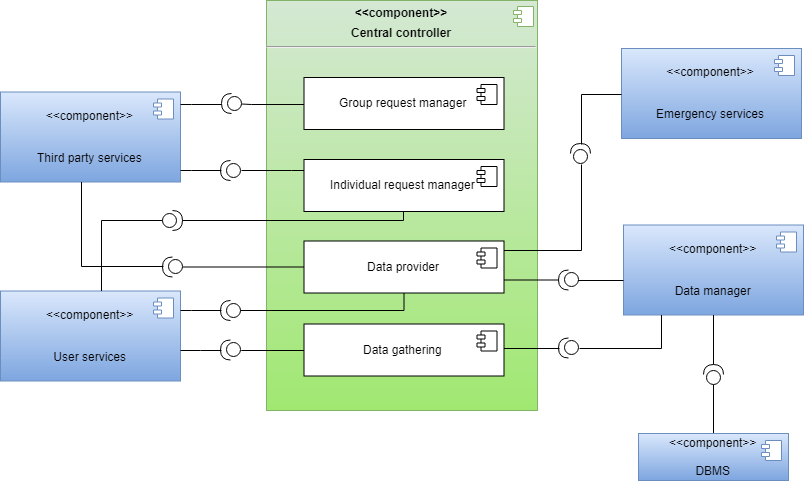
\includegraphics[width=300pt]{images/CompView/Component_view2.png}
    \caption{High Level Components.}
\end{figure}
\noindent The Central Controller is the core of the system, it's modules manage the acquisition, storing and exchange of data between users and third parties:
\begin{itemize}
    \item \textbf{Group request manager}: this module contains the logic concerning group requests. After receiving a request from a third party, it checks that the privacy condition is respected and authorizes or forbids the access to data.
    \item \textbf{Individual request manager}: this module receives the individual requests and forwards them to the corresponding user. After receiving the response from the recipient it authorizes or forbids the access to data.
    \item \textbf{Data provider}: service that provides users' data to authorized applicants.
    \item \textbf{Data gathering}: module that receives users' data and stores them by using the Data Manager component.
\end{itemize}
\clearpage
\hypertarget{ES}{}
\begin{figure}[ht]
    \centering
    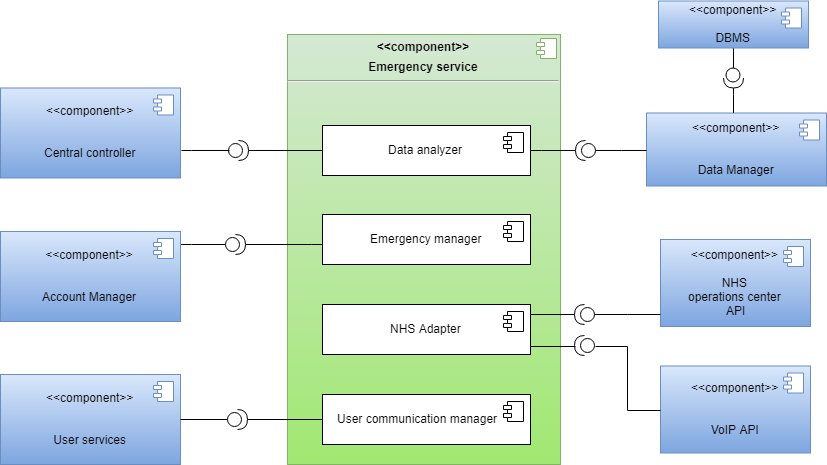
\includegraphics[width=300pt]{images/CompView/Component_view3.png}
    \caption{High Level Components.}
\end{figure}
\noindent The Emergency Service is the component that manages the logic behind AutomatedSOS.
Since this application is built on top of Data4Help, the emergency service is conceived as a stand-alone module inside the back-end logic of the system.
AutomatedSOS exploits Data4Help technology to obtain users' data from the Data Provider of central controller.
The two systems share the same Account Manager, so every user that registers to AutomatedSOS is also a Data4Help user. 

\begin{itemize}
    \item \textbf{Data analyzer}: connects to the central controller to acquire users' data and analyzes them in real time. This module also connects to the Data Manager to obtain the parameters thresholds.
    \item \textbf{Emergency Manager}: if the data analyzer detects an anomaly, it alerts the Emergency Manager. This module creates an emergency message containing the user personal credentials, its current position and most recent health parameters.
    \item \textbf{NHS Adapter}: this module sends the message generated by the Emergency Manager, adapting it to the interface provided by the National Health Service or making an automatic call to the Operations Center using the VoIP protocol if the NHS doesn't provide an API in the hosting country.
    \item \textbf{User Communication manager}: this module is responsible for the communication between AutomatedSOS and the user. If the user is having a health emergency, the Communication Manager notifies him about the ambulance arrival.
\end{itemize}
\clearpage
\section{Deployment	View}
In this section we illustrate the deployment of the system components on the hardware infrastructure.
The design of the hardware architecture was made keeping in mind the non-functional requirements illustrated in the RASD document. The objective was to obtain a reliable and scalable system, but also to avoid an over-complicated disposition, that would increase the costs of construction and maintenance. \\
We chose to deploy the system using a four tiers architecture:
\begin{itemize}
    \item the \textbf{first tier} represents the client applications:\\the system will be accessible by smartphones, wearables and web browsers. All these platforms will exchange messages using the HTTP protocol. There will be two different apps for Android and iOS, implemented using the native frameworks of the operating systems. We made the decision to avoid cross platform development solutions to build the client apps, because they will be a very small portion of the code base and will provide only presentation services. Both applications will connect to the same interfaces provided by the system. We also chose to avoid other mobile platforms, since the current scenario in mobile OS clearly shows a duopoly of two competitors that will unlikely change in the next years.
    The web client will be developed using HTML5 and CSS for the design and JavaScript for the web page logic.
    \item in the \textbf{second tier} will be placed the web server:\\implemented using an Apache HTTP architecture, it will be responsible  for the communications with web browsers.
    \item the \textbf{third tier} will be the core of the system:\\two application servers will contain Data4Help and AutomatedSOS central logic. They will be based on Glassfish\cite{GlassFish}, the reference implementation by Oracle of Java EE\cite{JEE} specifications. The use of JEE promotes the creation of a multi-platform ("Write Once, Run Anywhere"), portable and scalable central system.
    In particular, Glassfish offers complete support to Enterprise JavaBeans, JMS, RMI and other JEE key features. Furthermore, this platform provides robust off-the-shelf mechanisms to support the interoperability with non Java systems (JAX-WS, JAX-RS).
    \item the \textbf{fourth tier} will be occupied by the Databases:\\all the the data will be stored using Oracle DBMS and backup database servers. The application servers and the database will interact using the JDBC protocol.
\end{itemize}

\noindent Every tier will be isolated from the others with the use of a firewall. The application servers, that are the most sensitive components of the architecture, will be deployed inside a demilitarized zone.\\
In the next page is presented a deployment diagram that models the proposed architecture.
\begin{landscape}
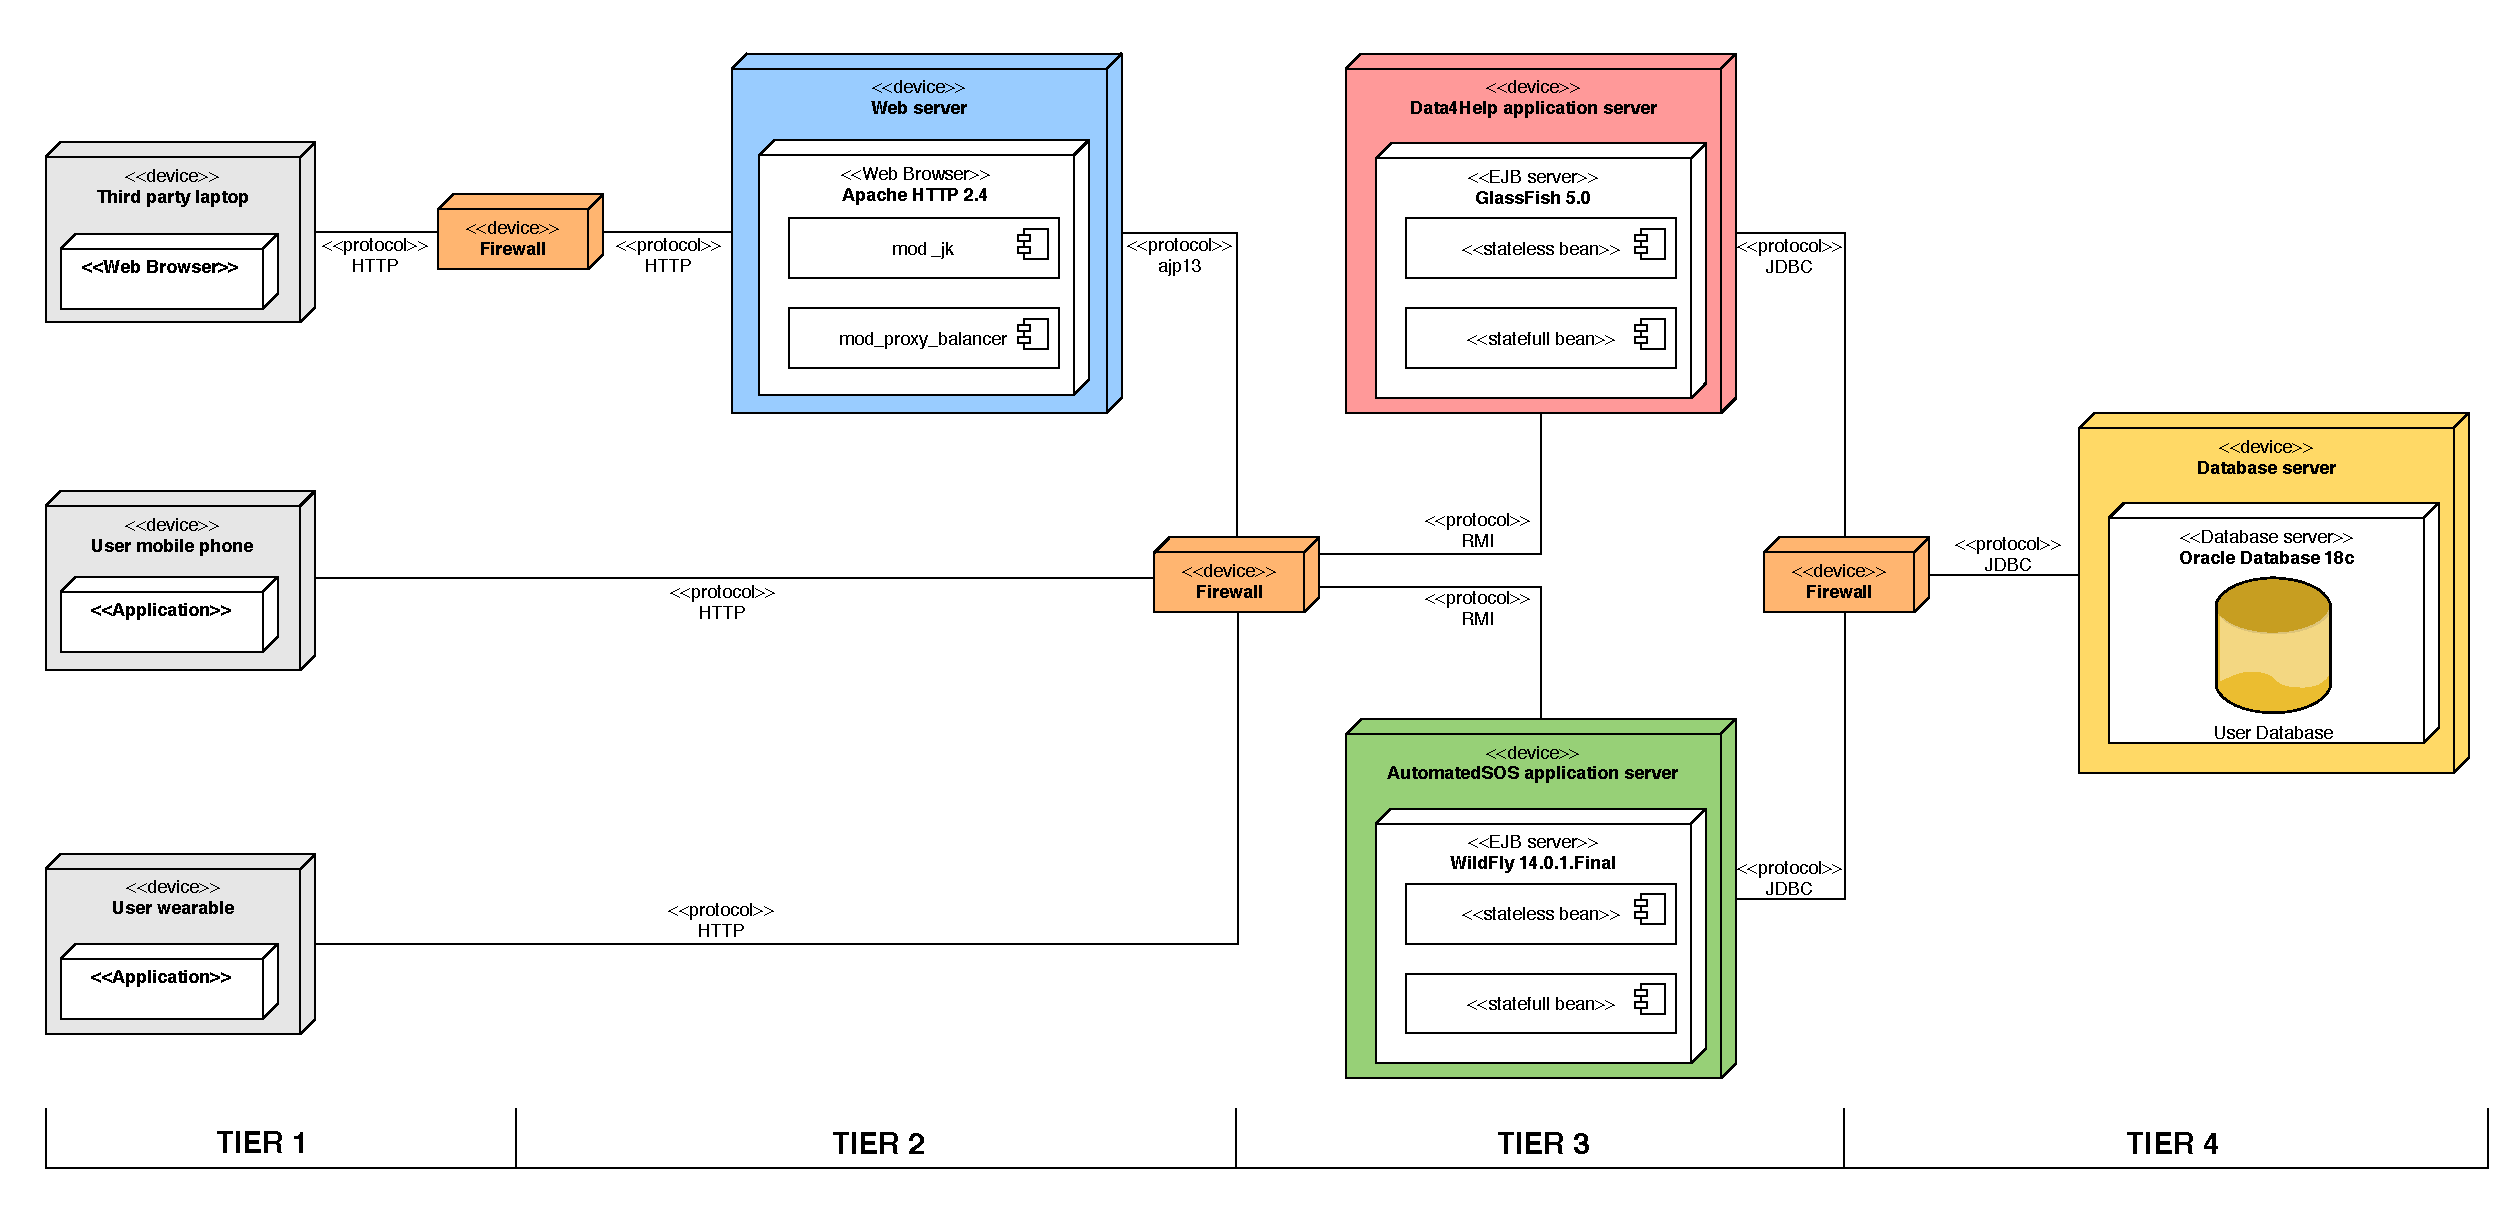
\includepdf[angle=90]{pdfs/Deployment_view.pdf}
\end{landscape}

\hypertarget{RV}{\section{Runtime View}}
This section illustrates the phases of the main interactions that happen during the use of the system. Using several Sequence Diagrams, we illustrated the communications between the logic components.\\
Even though we tried to describe the processes in the most clear and detailed way, these diagram remains a high-level description of the interactions flows. Therefore, all of the parameters and methods that appear in these Sequence Diagrams may do not correspond exactly to the ones in the actual implementation of the components.\\
In the following Sequence Diagrams we cover all the possible interactions between each component. We grouped all the Sequence Diagram that belong to the same flow of activities, since for obvious reasons we had to decomposed them in sub-sequence to fit them into this document.
The diagrams presented below cover all these situations:
\begin{itemize}
    \item Registration of a user (which is identical to the registration of a third party, so we omit this last one) : \underline{Figure \ref{RV1}}
    \item Login of a user (which is identical to the login of a third party, so we omit this last one) : \underline{Figure \ref{RV2}}
    \item A third party makes an individual request :\\ \underline{Figure \ref{RV1}}, \underline{Figure \ref{RV3}}, \underline{Figure \ref{RV4}}, \underline{Figure \ref{RV5}}, \underline{Figure \ref{RV6}}, \underline{Figure \ref{RV7}}
    \item A third party makes a group request :  \underline{Figure \ref{RV8}}
    \item AutomatedSOS analyzes health parameters and detects an anomaly:\\ \underline{Figure \ref{RV9}},  \underline{Figure \ref{RV10}},  \underline{Figure \ref{RV11}}
    
\end{itemize}

\begin{figure}[ht]
    \makebox[\textwidth]{
        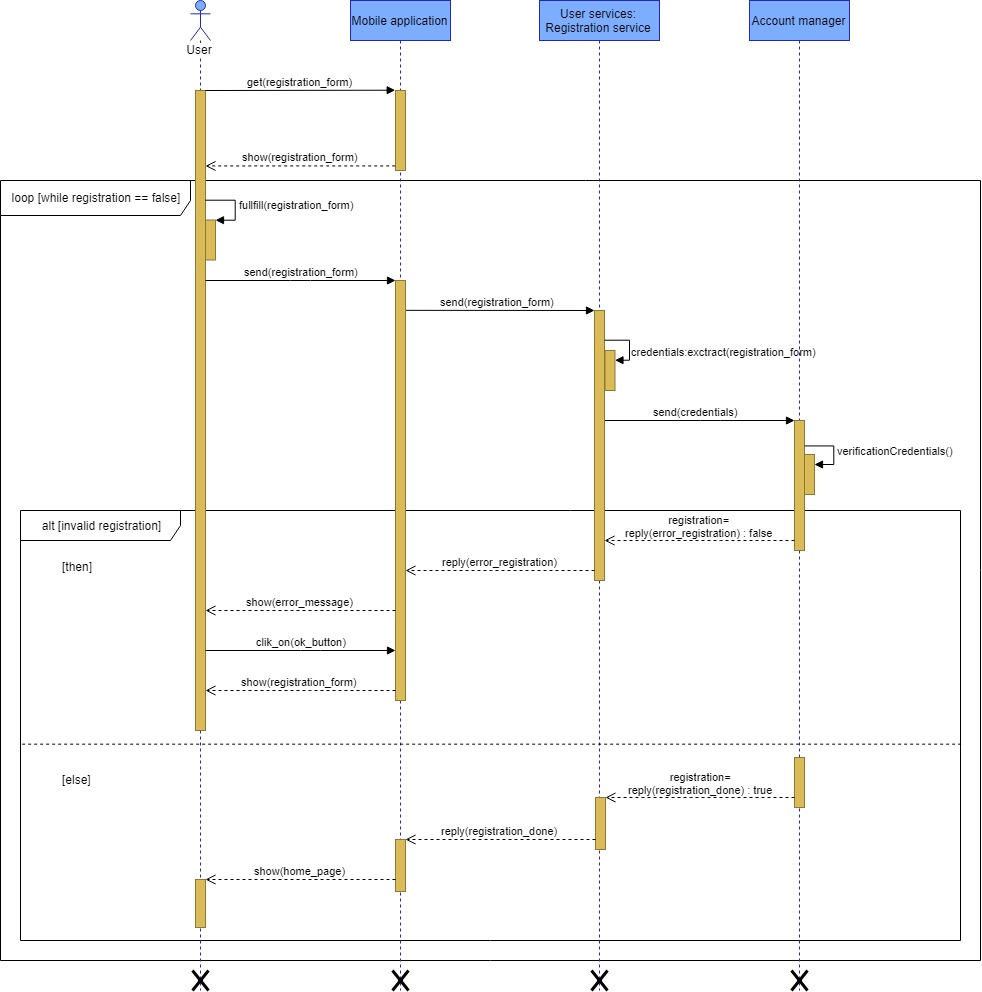
\includegraphics[width=1.3\linewidth]{images/RuntimeDiagrams/Registration.jpg}
    }
    \caption{Data4Help - Registration of a user.}
    \label{RV1}
\end{figure}

\begin{figure}[ht]
    \makebox[\textwidth]{
        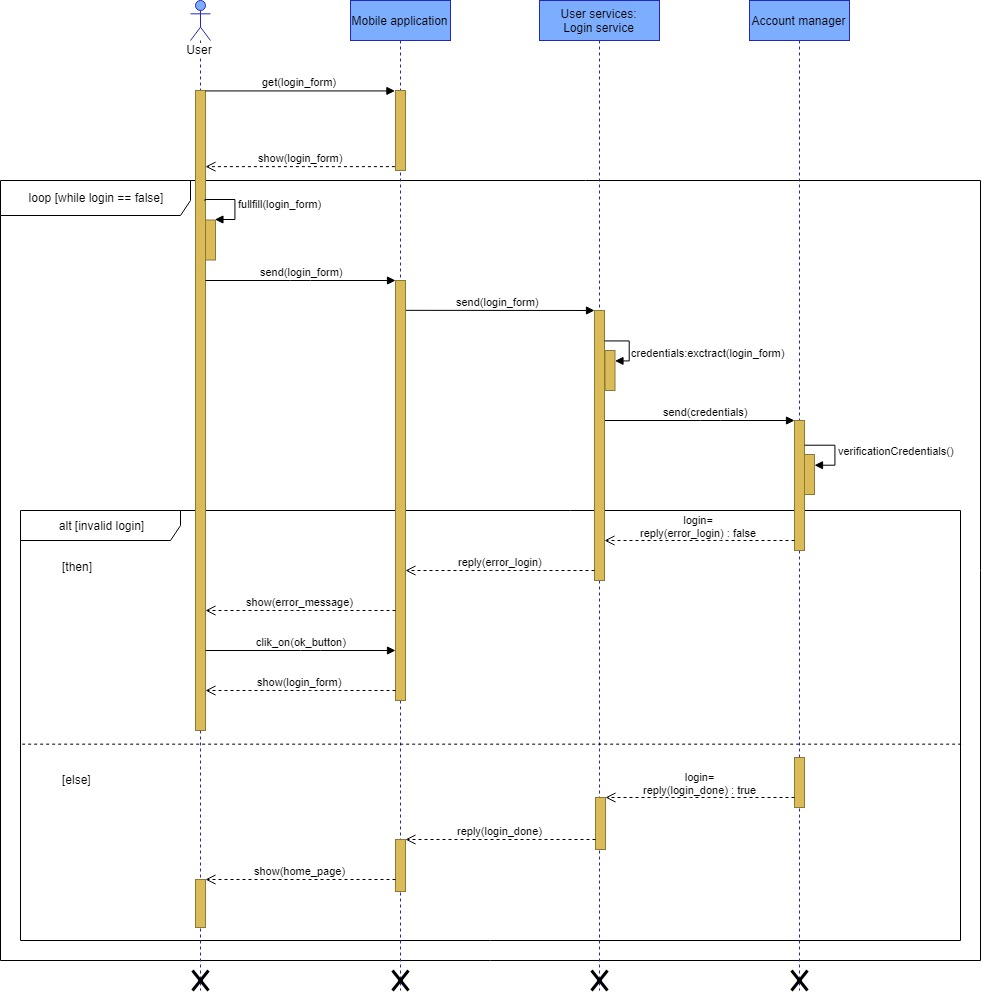
\includegraphics[width=1.3\linewidth]{images/RuntimeDiagrams/Login.jpg}
    }
    \caption{Data4Help - Login of a user.}
    \label{RV2}
\end{figure}

%individual request(from here)
\begin{figure}[ht]
    \makebox[\textwidth]{
        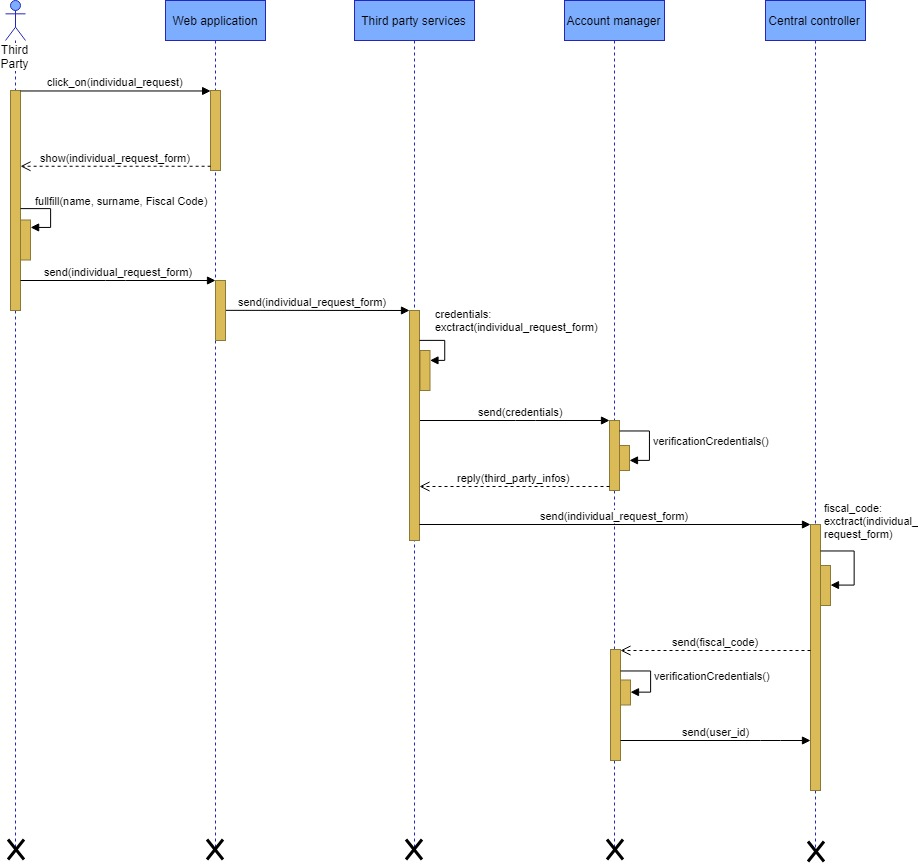
\includegraphics[width=1.3\linewidth]{images/RuntimeDiagrams/IndividualRequest1.jpg}
    }
    \caption{Individual request - A third party makes an individual request.}
    \label{RV3}
\end{figure}

\begin{figure}[ht]
    \makebox[\textwidth]{
        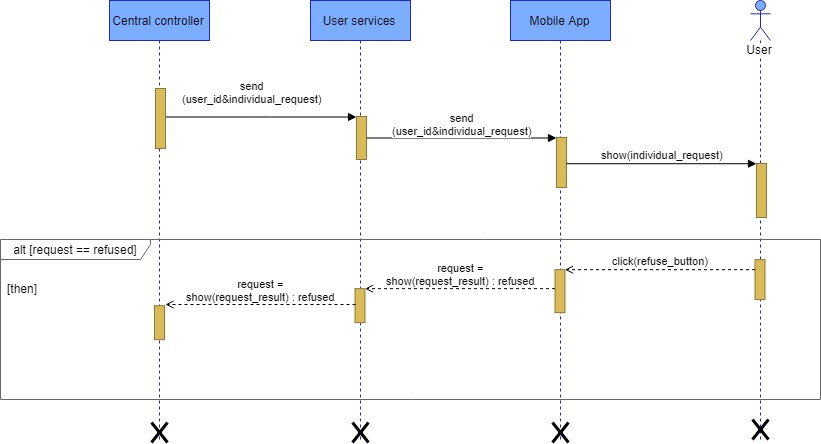
\includegraphics[width=1.3\linewidth]{images/RuntimeDiagrams/IndividualRequest2.jpg}
    }
    \caption{Individual request - The individual request is forwarded to the user and he/she refuses it.}
    \label{RV4}
\end{figure}

\begin{figure}[ht]
    \makebox[\textwidth]{
        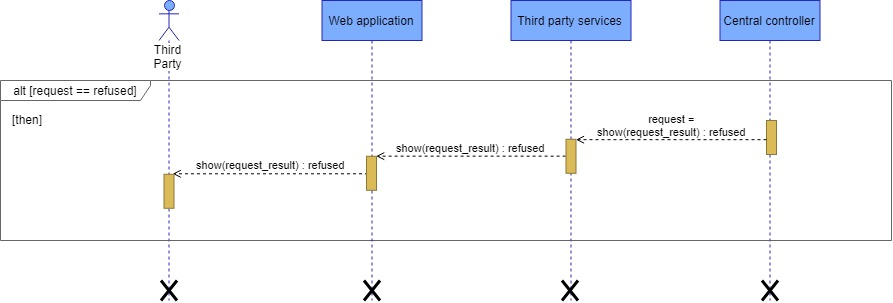
\includegraphics[width=1.3\linewidth]{images/RuntimeDiagrams/IndividualRequest3.jpg}
    }
    \caption{Individual request - The reply is sent to the third party.}
    \label{RV5}
\end{figure}

\begin{figure}[ht]
    \makebox[\textwidth]{
        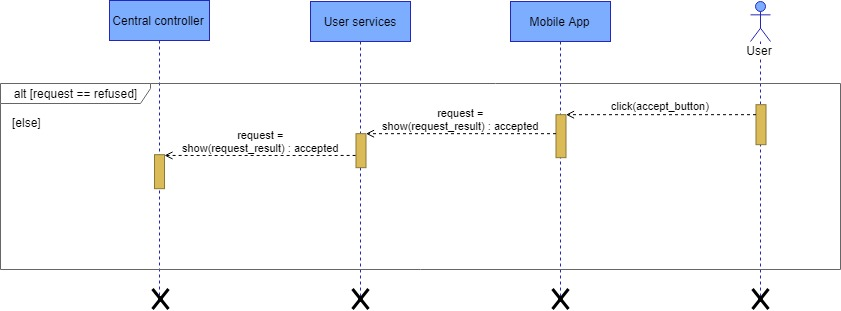
\includegraphics[width=1.3\linewidth]{images/RuntimeDiagrams/IndividualRequest4.jpg}
    }
    \caption{Individual request - The user accepts the request.}
    \label{RV6}
\end{figure}

\begin{figure}[ht]
    \makebox[\textwidth]{
        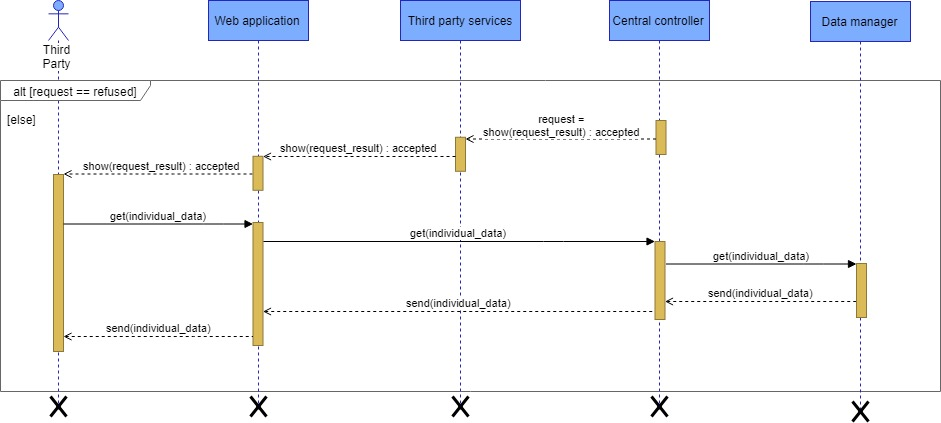
\includegraphics[width=1.3\linewidth]{images/RuntimeDiagrams/IndividualRequest5.jpg}
    }
    \caption{Individual request - The reply and the individual data are sent to the third party who requested them.}
    \label{RV7}
\end{figure}
%individual request(up to here)

\begin{figure}[ht]
    \makebox[\textwidth]{
        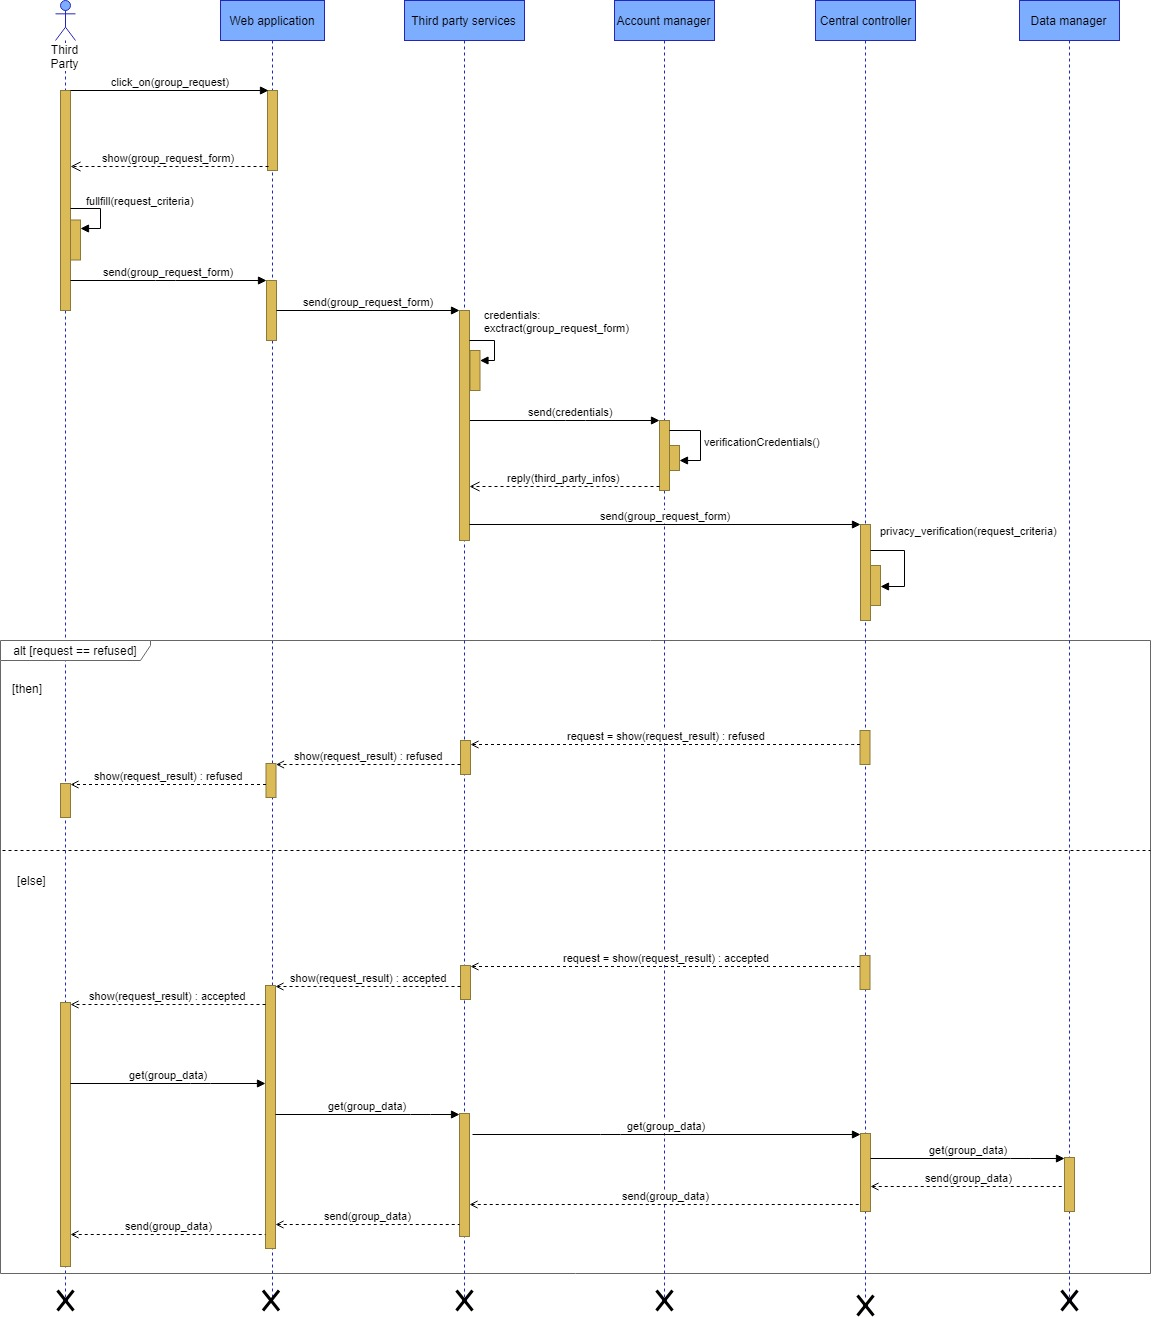
\includegraphics[width=1.3\linewidth]{images/RuntimeDiagrams/GroupRequest.jpg}
    }
    \caption{Data4Help - A third party makes a group request.}
    \label{RV8}
\end{figure}

\begin{figure}[ht]
    \makebox[\textwidth]{
        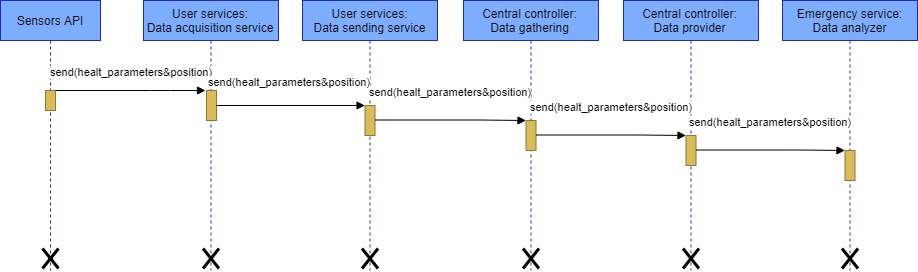
\includegraphics[width=1.3\linewidth]{images/RuntimeDiagrams/Ambulance1.jpg}
    }
    \caption{AutomatedSOS - Real-time data acquisition.}
    \label{RV9}
\end{figure}

\begin{figure}[ht]
    \makebox[\textwidth]{
        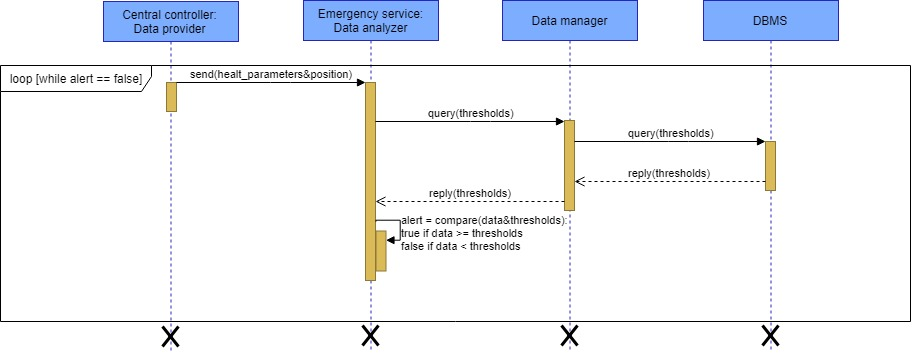
\includegraphics[width=1.3\linewidth]{images/RuntimeDiagrams/Ambulance2.jpg}
    }
    \caption{AutomatedSOS - Real-time data analysis.}
    \label{RV10}
\end{figure}

\begin{figure}[ht]
    \makebox[\textwidth]{
        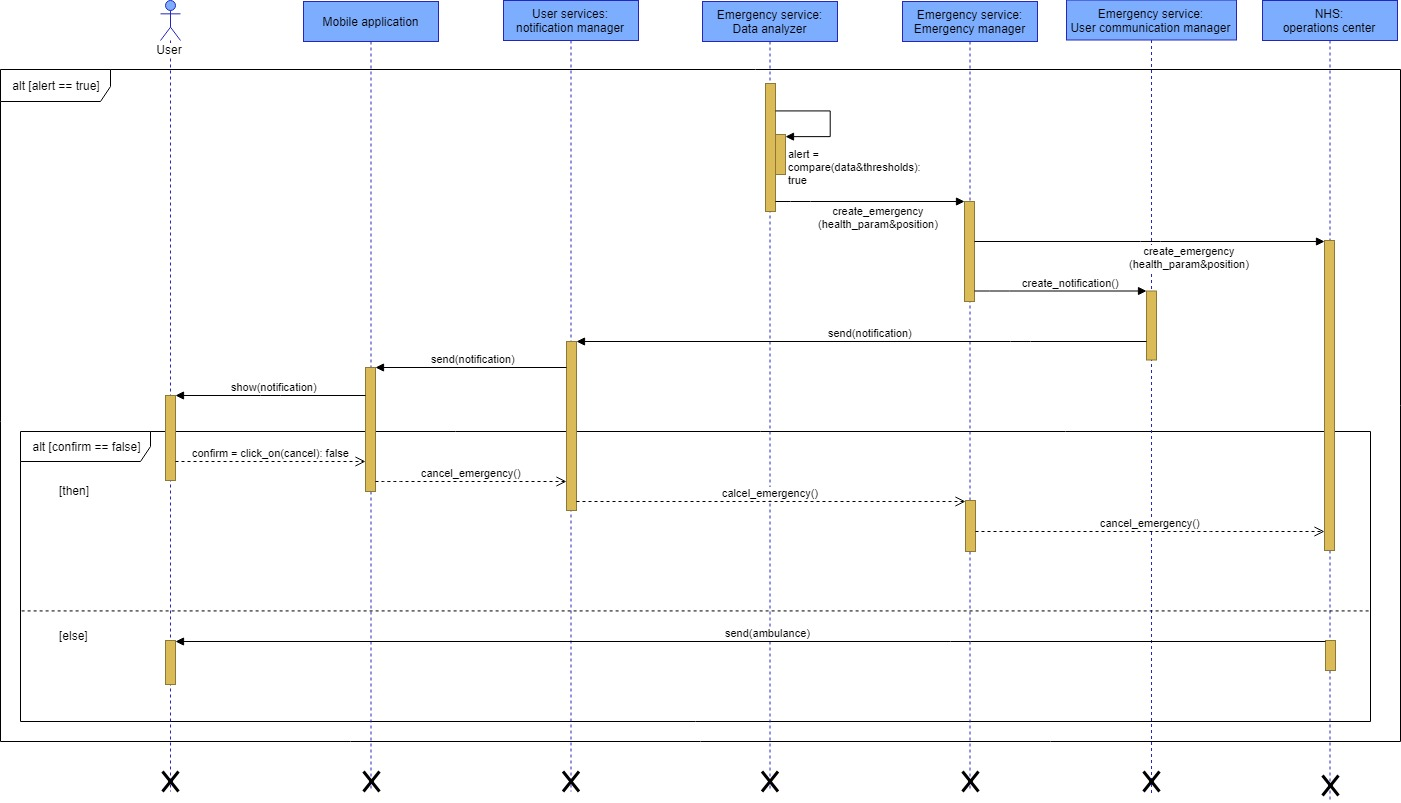
\includegraphics[width=1.3\linewidth]{images/RuntimeDiagrams/Ambulance3.jpg}
    }
    \caption{AutomatedSOS - An emergency is detected.}
    \label{RV11}
\end{figure}

\clearpage
\section{Component Interfaces}
The diagrams showed below list the main methods that form the components interfaces.\\
Since the Central Controller behaves as an intermediary between users (collection of data) and third parties (transfer of these data), the component provides interfaces that serve the communication with both parties.
In particular, the Individual Request Manager offers methods for the addition of a request by a third party and the response to that request by the user. \\
The Third Party and User services offer all the methods responsible for the interaction between the client applications and the back-end. Thanks to these components, all the different implementations of the presentation tier can interact with the same interface.\\
Examples of methods offered by the Third Party Services regards the sending of a request and the access to users' data. Examples of methods offered by the User Services regards the response to an incoming request and the data acquisition from the device.\\
The emergency service provides the methods to collect and analyze health data, generate and send emergency notification to the NHS and communicate with the user.\\
\clearpage

\begin{figure}
    \centering
    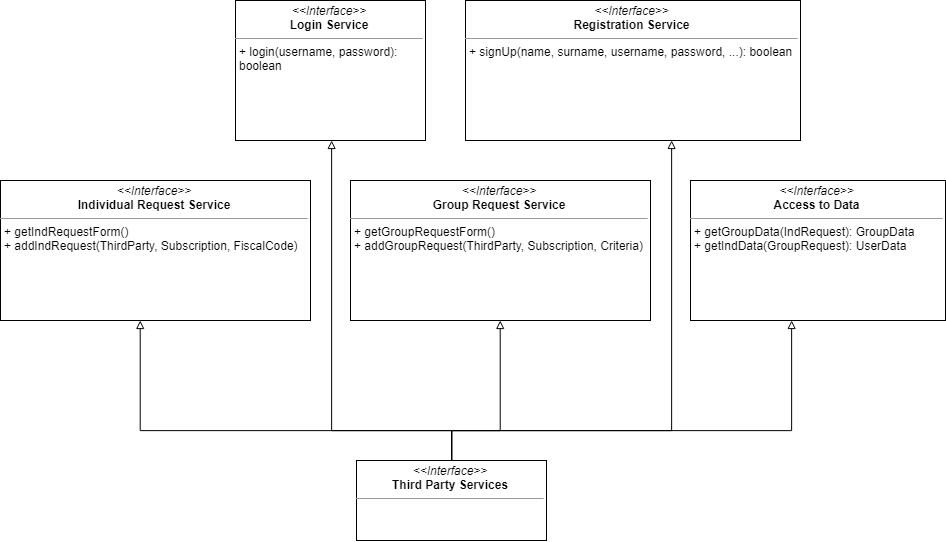
\includegraphics[width=300pt]{images/CompInterfaces/Component_interfaces3.png}
    \caption{Component Interface}
\end{figure}

\begin{figure}
    \centering
    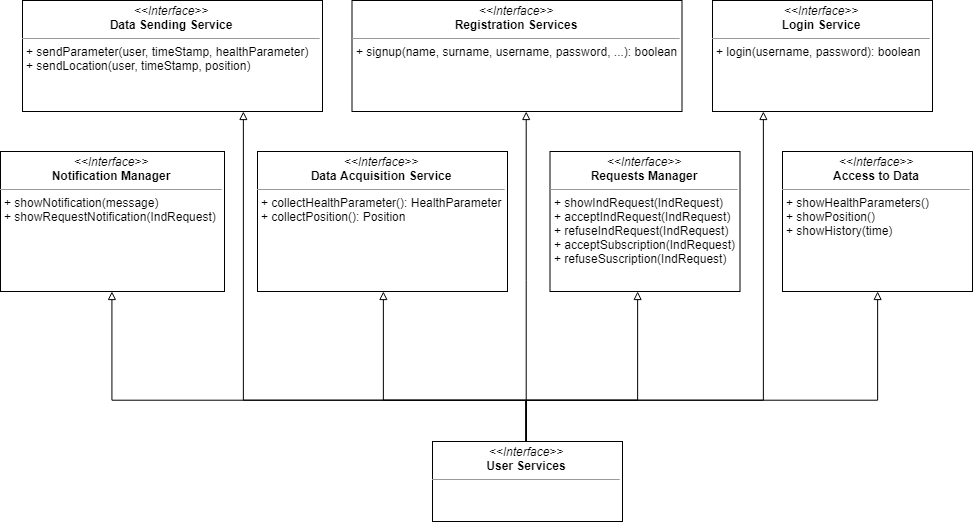
\includegraphics[width=300pt]{images/CompInterfaces/Component_interfaces4.png}
    \caption{Component Interface}
\end{figure}


\begin{figure}
    \centering
    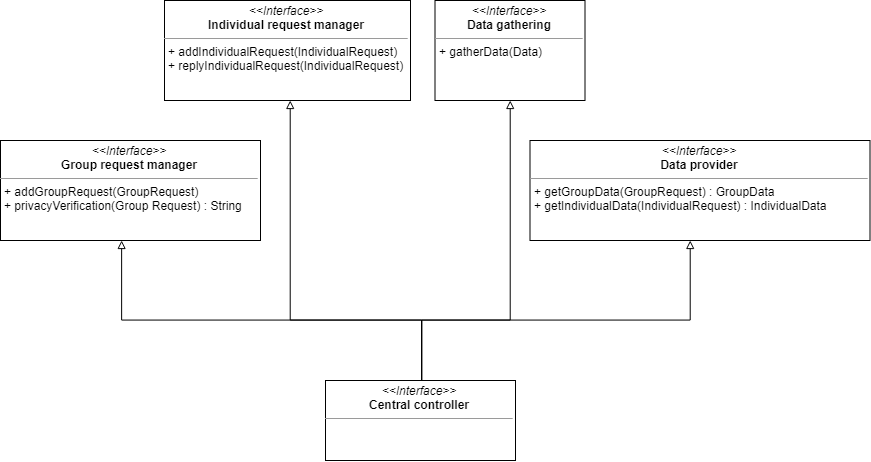
\includegraphics[width=300pt]{images/CompInterfaces/Component_interfaces1.png}
    \caption{Component Interface}
\end{figure}

\begin{figure}
    \centering
    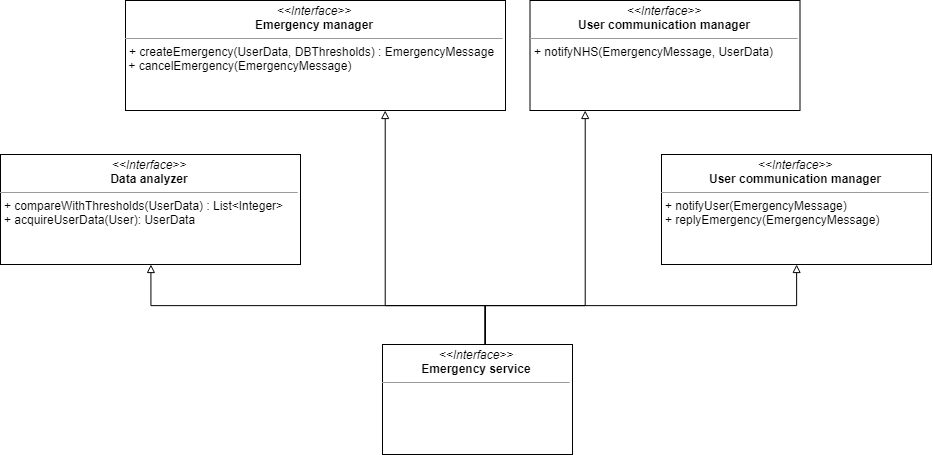
\includegraphics[width=300pt]{images/CompInterfaces/Component_interfaces2.png}
    \caption{Component Interface}
\end{figure}


\clearpage

\hypertarget{Arch_Patt}{\section{Selected Architectural Styles and Patterns}}
\begin{itemize}
    \item \textbf{Model-View-Controller:} it's a very common design pattern, that separates the architecture into three communicating components. The Controller performs actions on the Model, using inputs from the View. The Model contains the application data structures and the View gives an external representation of them.\\ 
    The MVC pattern promotes the code reuse and avoids the coupling between data and their representation. This pattern is particularly appropriate for complex systems such as Data4Help and AutomatedSOS, that will be deployed in multiple physical nodes and will provide several types of views to their users.  
    \item \textbf{\hypertarget{SOA_TG}{Service Oriented Architecture:}} we designed the system components as a set of services that interacts with each other through a communication protocol. Viewing each component as a service gives the advantages of abstracting its functions to the highest level and see the module as a independent black box.\\
    A SOA enhances the modularity and maintainability of the system. It also promotes the creation of robust and complete interfaces for each component.
    \item \textbf{Proxy Pattern and Facade Pattern:} we used these patterns mainly for the interactions between the back-end and the client applications. The proxy pattern provides an intermediate object that substitute for the real subject of a communication, while controlling that the input is valid and the access is appropriate. The facade pattern implements a simple interface for the access of the back-end system and also acts as an adapter for the information exchanges in the messages. We used these patterns to create an interface between clients and the central system that could be simple to access, secure and that could minimize the dependencies between modules.
    \item \textbf{Publish/Subscribe Pattern:} it is closely related to the MVC pattern. This architectural style offers great scalability and it's fundamental to ensure satisfying performances in an event-based system. This pattern allows to send users' data as soon as they are collected and to notify an emergency as soon as it's detected. 
    \item \textbf{Factory pattern (software design pattern):} a factory object provides a public method for creating other objects, while hiding the actual creation process. The factory pattern promotes the overall encapsulation in the code base.
    \item \textbf{Strategy pattern (software design pattern):} allows the creation of a set of encapsulated algorithms and the selection of one of them at run-time. This pattern is one of the most common in OOP and promotes encapsulation and polymorphism.
    \item \textbf{Adapter pattern (software design pattern):} used to adapt two different interfaces. This pattern is particularly useful for the integration between AutomatedSOS and the NHS of the hosting country. A more detailed description of its usage will be given in the next paragraph. 
\end{itemize}

\section{Other Design Decisions}

\begin{itemize}
    \item \textbf{Google Maps API:} to represent current positions and daily routes we will use the maps API offered by Google. This API is the common standard because of its quality and current updates. Google Maps offers an interface for JavaScript\cite{mapsAPI-JS}, Android\cite{mapsAPI-Android} and iOS\cite{mapsAPI-iOS} development.
    \item \textbf{Sensors API and healthKit:} to collect data from users' device we will exploit the APIs offered by Android and iOS platforms: Sensors API\cite{sensorsAPI} and healthKit\cite{healthKit}.
    \item \textbf{AutomatedSOS and Data4Help integration:} when designing AutomatedSOS, we followed two main guide lines: promoting the code reuse as much as possible and keeping the central logic of the application independent from Data4Help's components.
    Given these objectives, we designed AutomatedSOS as an independent service, built on-top of Data4Help platform. 
    The two apps share the same account management system, so whenever a user registers to AutomatedSOS he/she also becomes a Data4Help user.\\
    AutomatedSOS core module (\hyperlink{ES}{ \underline{Emergency Service}}) exploits Data4Help's Data Provider to obtain users' data in real time.
    Placing the logic of the two systems in distinct modules favors a distributed deployment of the back-end and a correct load balance.
    In terms of reliability, a failure in AutomatedSOS does not affect Data4Help operations (the vice versa is not true, for obvious reasons).
    \item \hypertarget{NHS_API}{\textbf{Interaction with the NHS:}} AutomatedSOS will be hopefully adopted in several countries, that have significantly different National Health Institutions, First Aid services and unit of measurement for the health parameters.\\
    An efficient integration between the system and the local NHS is a fundamental requirement for the success of an application that deals with its users' lives.\\
    The existence of many differences between the countries forces the design to be adapted to each specific NHS. In order to do so, the NHS Adapter is the interface component responsible for the translation between the system and the local Operations Center.
    To give an high-level description: if a country offers an API to send a digital message to the Operations Center, the NHS Adapter will connect to it; if such an API does not exists, the NHS adapter will call 911 (112 in Italy) telephone number and read the emergency message to the operator with an artificial voice.
\end{itemize}